\documentclass[en]{../../../../../../eplexam}

\usepackage{pgfplots}
\pgfplotsset{compat=1.15}
\pdfminorversion=7

\hypertitle{Secure electronic circuits and systems}{8}{ELEC}{2760}{2019}{Juin}{All}
{Martin Braquet \and Romain Pattyn}
{François-Xavier Standaert}

During the written exam, it is possible to present/explain/detail on demand one (or both) question(s) to the professor.

\section{}
We consider the following Sbox:
$$S_{box}(a(x))=x\cdot\left(a(x)^{-1}\right) \mod p(x)$$
where $p(x) = x^4\oplus x\oplus 1$ to bring the output back in GF$(2^4)$.
\begin{enumerate}
    \item Implement the inverse as a function of products and squares only. Try to minimise the amount of such function calls because we will later use masking. Remember that $x^{-1} = x^{p^m-2}$ in GF$(p^m)$
    \item Why do we say that the square operator is $\oplus$-linear in a function characteristic 2. (hint: start by checking at $(x^2\oplus 1)^2 \mod p(x)$ and generalise it to any sum of polynomials.)
    \item Why can we say the same thing about the multiplication by the constant polynomial $c(x) = x$? (recall that this is equivalent to the XTime table of the exercise session)
    \item Build the table squaring table.
    \item By using an FPGA with logic blocks similar as the LB1 of the course (2 LUT of 4 bit, one multiplexer and 2 registers) what is the cost of the implementation in LB1 of the squaring table and the multiplication table? You can consider that you have access to those tables, for the square operator you have an $n$-bit by $n$-bit table and for the multiplication operator you have an $n_1$-bit by $n_2$-bit table.
    \item We want to mask the data with 3 shares, how many calls to the previous table implementations would you have to do for the square and multiplication operator?
\end{enumerate}

\nosolution

\section{}

Consider an encryption scheme where the Sbox is composed of a nonlinear function followed by a squaring operator. The output of the Sbox is then classically xored with the key. All the variables are expressed as 4-bit data (in GF($2^4$)).

\begin{figure}[H]
    \centering
    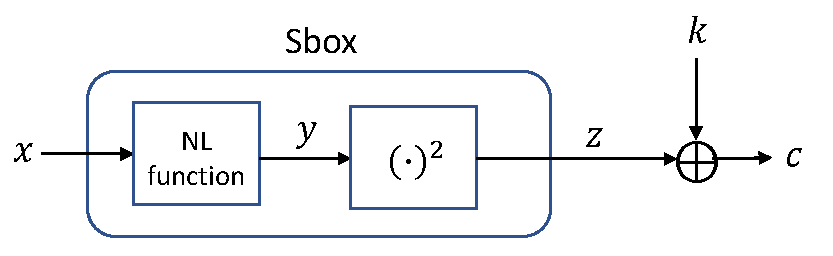
\includegraphics[width=0.6\textwidth]{Q2.pdf}
\end{figure}

\begin{enumerate}
    \item Is it possible to retrieve the key by inserting a toggling bit fault on $y$? If yes, how? If no, why?
    \item How many faults do we need to find the key by inserting a toggling bit fault on $x$ (i.e. a random bit of $x$ is toggled? The full encryption of a 128-bit key is composed of 32 encryption schemes in parallel, how many faults are required to find the full key? Explain.
    \item Now consider that the fault model is not so precise, so the fault toggles 2 random bits of $x$. How many faults are then needed to recover $k$? Explain your answer with theoretical information arguments. Hint: $C(4,2)=\binom{4}{2} = 6$ and $\log_2(6) \simeq 2.5$.
    \item \label{QL}
    We have at our disposal the (non-noisy) leakage $L$ of the 2 first bits of $z$: $L(z)="z_1z_0"$ ($z_i$ represents the $i$-th bit of $z$). How many encryptions do we need to recover the key?
    \item We have now at our disposal the (non-noisy) leakage $L$ of the 2 first bits of $x$: $L(x)="x_1x_0"$. The output\footnote{These numbers are given as an example, they were different in the exam.} of the Sbox is $$ [4,7,15,1,2,0,12,6,9,8,11,14,3,5,10,13].$$ Compute the key knowing that $c=0$ when $L="00"$, $c=1$ when $L="01"$ and $c=2$ when $L="11"$. 
    \item Which one of these (in)equalities is correct? Explain.
    \begin{align*}
        MI(x;L) & \le MI(k;L,c) \\
        MI(x;L) & =   MI(k;L,c) \\
        MI(x;L) & \ge MI(k;L,c)
    \end{align*}
    \item Compute $MI(x;L)$. Considering that $c=4$ in the formula given in the slides, compute the number of samples required to find the key. Is it in accordance to your answer of question \ref{QL}?
\end{enumerate}

\nosolution

\end{document}
